% ============================================================================
% SECTION 4: EXPERIMENTS
% ============================================================================
\section{Experiments}
\label{sec:experiments}

% ----------------------------------------------------------------------------
% 4.1 Main Robustness Results
% ----------------------------------------------------------------------------
\subsection{Robustness Comparison}
\label{subsec:robustness}

Table~\ref{tab:main_results} presents the main robustness comparison across all evaluated models. We report clean accuracy and robust accuracy under PGD-10 and AutoAttack with $\eps = 8/255$.

\begin{table}[!t]
\centering
\caption{Main Robustness Results on CIFAR-10 ($\eps = 8/255$)}
\label{tab:main_results}
\begin{tabular}{lccccc}
\toprule
\textbf{Model} & \textbf{Defense} & \textbf{Params} & \textbf{Clean} & \textbf{PGD-10} & \textbf{AA} \\
\midrule
\multicolumn{6}{l}{\textit{CNN Models}} \\
ResNet-18 & None & 11.2M & 94.37 & 0.00 & -- \\
ResNet-18 & AT & 11.2M & 81.80 & 40.97 & \textbf{36.00} \\
WRN-28-10 & AT$^\dagger$ & 36.5M & 89.48 & 66.05 & 62.76 \\
\midrule
\multicolumn{6}{l}{\textit{Vision Transformer Models}} \\
ViT-Tiny & None & 5.7M & 77.50 & 0.00 & -- \\
ViT-Tiny & AT & 5.7M & 73.60 & 36.87 & \textbf{32.40} \\
\bottomrule
\multicolumn{6}{l}{\footnotesize $^\dagger$Pretrained model from RobustBench~\cite{croce2021robustbench}. AA = AutoAttack.}
\end{tabular}
\end{table}

The results reveal a consistent robustness advantage for CNNs under standard adversarial training. ResNet-18 AT achieves 36.0\% robust accuracy under AutoAttack, compared to 32.4\% for ViT-Tiny AT---a 3.6\% absolute gap despite the CNN having approximately twice as many parameters. The clean accuracy gap is 8.2 percentage points (81.8\% vs 73.6\%). Notably, AutoAttack robustness is consistently lower than PGD-10 robustness for both architectures (4.97\% drop for ResNet-18, 4.47\% drop for ViT-Tiny), confirming the importance of using this stronger benchmark for reliable evaluation. The WideResNet-28-10 baseline from RobustBench, achieving 62.76\% robust accuracy, demonstrates that model capacity plays a crucial role in adversarial robustness beyond architectural choice.

\begin{figure}[!t]
\centering
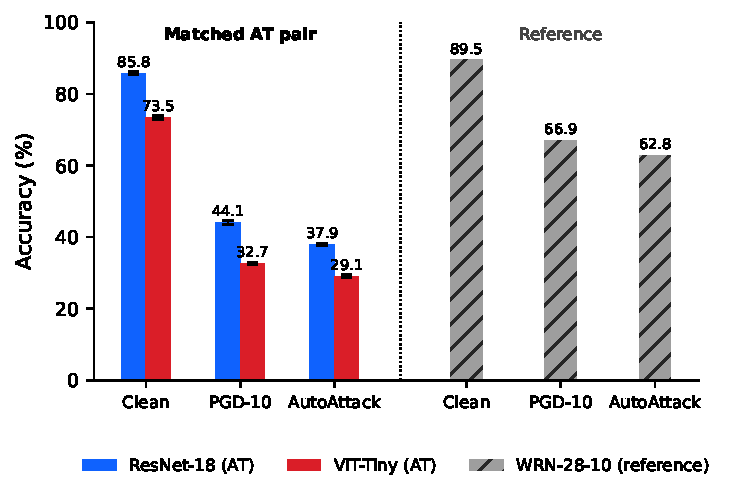
\includegraphics[width=\columnwidth]{../figures/final/fig1_robustness_comparison.pdf}
\caption{Robustness comparison across architectures under AutoAttack ($\eps=8/255$). CNNs consistently outperform ViTs under standard adversarial training, with WideResNet-28-10 achieving the highest robust accuracy due to its larger model capacity.}
\label{fig:robustness_comparison}
\end{figure}

Figure~\ref{fig:robustness_comparison} visualizes this robustness gap across architectures. To further understand the effect of perturbation magnitude, Figure~\ref{fig:epsilon_sweep} shows robust accuracy across different epsilon values.

\begin{figure}[!t]
\centering
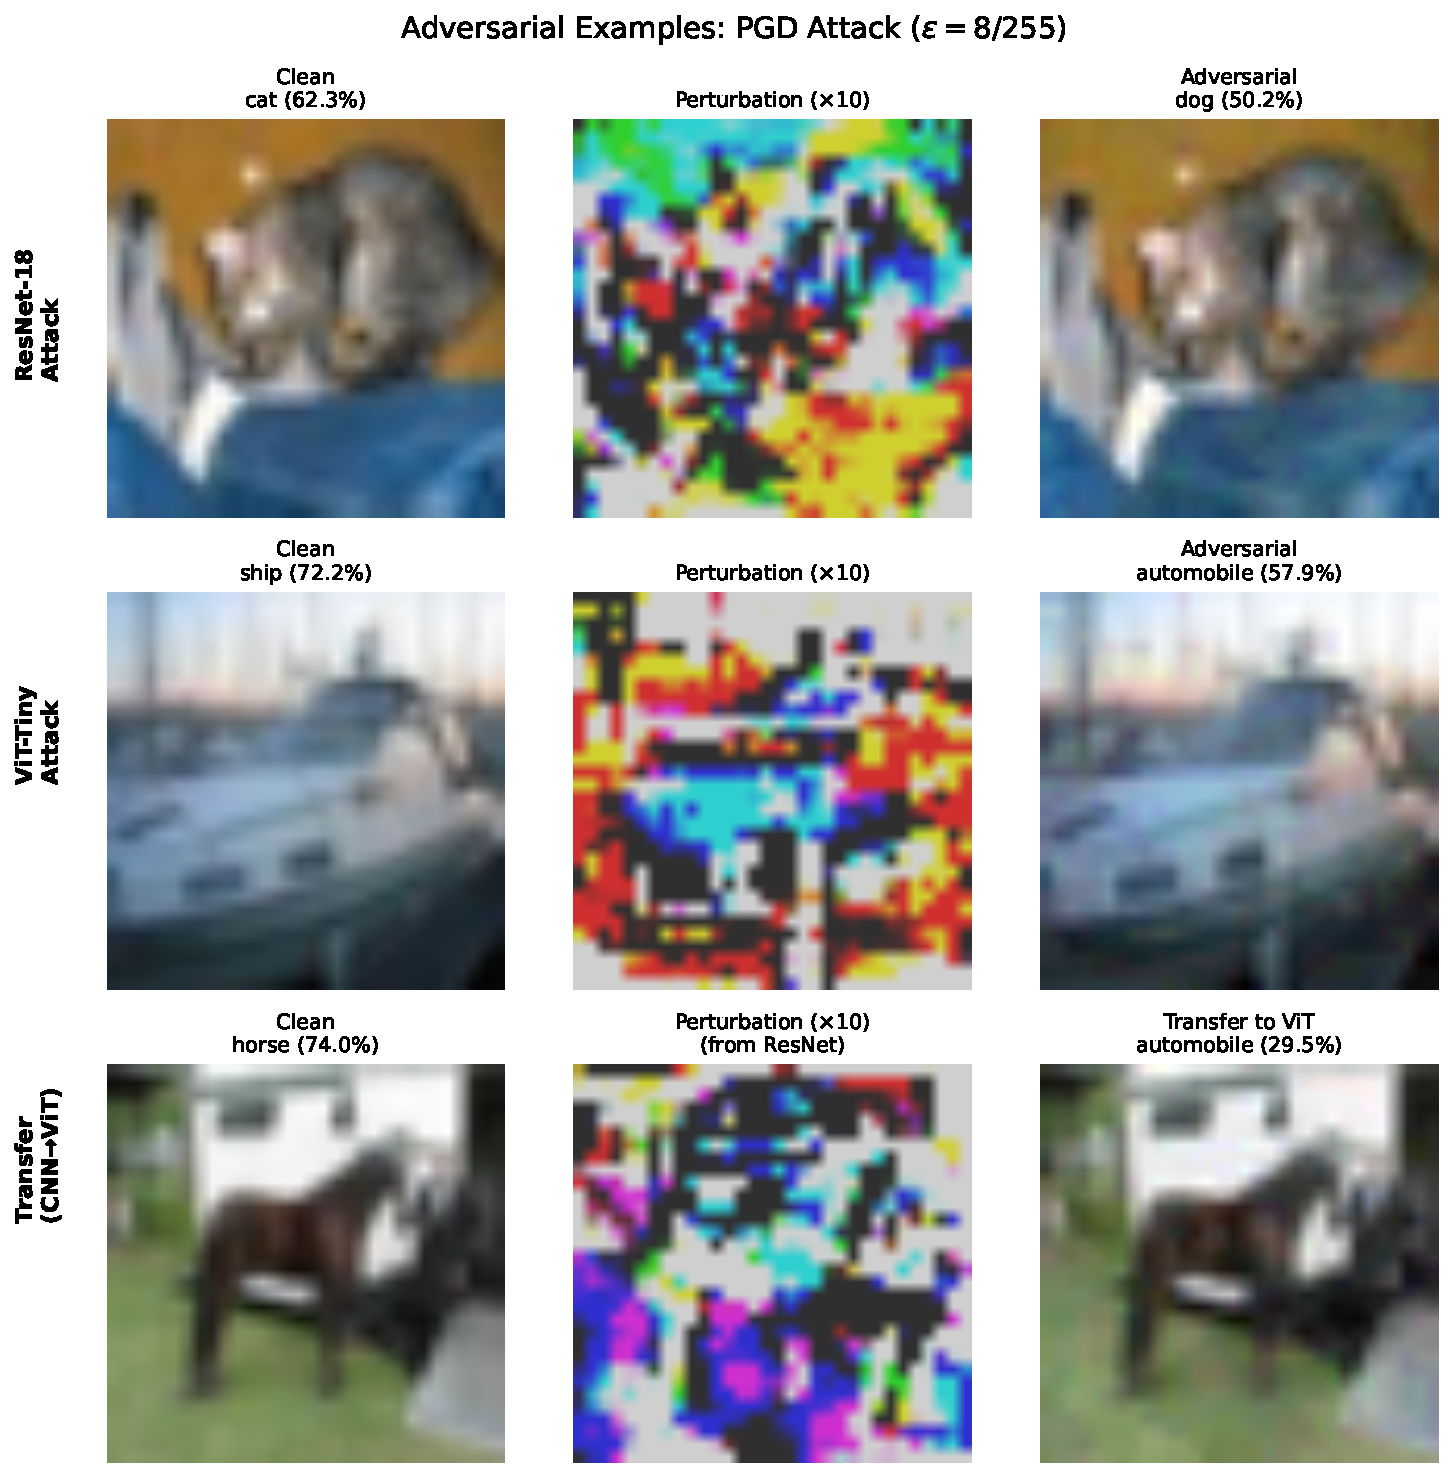
\includegraphics[width=\columnwidth]{../figures/final/fig_adversarial_examples.pdf}
\caption{Adversarial example visualization. Each row shows: original image with model prediction, perturbation magnified $10\times$, and adversarial image with new prediction. Row 1: Attack on ResNet-18. Row 2: Attack on ViT-Tiny. Row 3: Transfer attack (generated on ResNet, evaluated on ViT). The perturbations are imperceptible yet cause confident misclassifications.}
\label{fig:adversarial_examples}
\end{figure}

Figure~\ref{fig:adversarial_examples} provides visual examples of adversarial perturbations and their effects on model predictions.

\begin{figure}[!t]
\centering
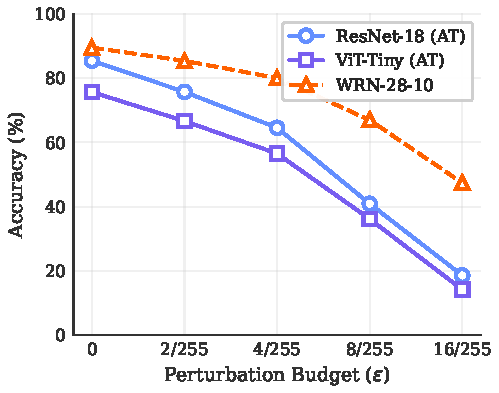
\includegraphics[width=\columnwidth]{../figures/final/fig2_epsilon_sweep.pdf}
\caption{Robust accuracy vs. perturbation budget ($\eps$). Both architectures exhibit similar degradation patterns as epsilon increases.}
\label{fig:epsilon_sweep}
\end{figure}

% ----------------------------------------------------------------------------
% 4.2 Transfer Attack Analysis
% ----------------------------------------------------------------------------
\subsection{Transfer Attack Analysis}
\label{subsec:transfer}

We analyze the transferability of adversarial examples between architectures using PGD-10 attacks. Table~\ref{tab:transfer} shows the transfer attack success rate matrix, where adversarial examples are generated on the source model (rows) and evaluated on the target model (columns).

\begin{table}[!t]
\centering
\caption{Transfer Attack Matrix. Source model (row) generates adversarial examples, evaluated on target model (column). White-box attack success rate shown on diagonal. Results computed over 1,000 test samples.}
\label{tab:transfer}
\begin{tabular}{lcc}
\toprule
\textbf{Source} $\rightarrow$ \textbf{Target} & \textbf{ResNet-18 AT} & \textbf{ViT-Tiny AT} \\
\midrule
ResNet-18 AT & 59.9\% & \textbf{41.2\%} \\
ViT-Tiny AT & \textbf{36.1\%} & 62.7\% \\
\bottomrule
\end{tabular}
\end{table}

As defined in Section~\ref{subsec:metrics}, the transfer attack success rate measures the misclassification rate of the target model on adversarial examples crafted against the source model (computed over all test samples). The off-diagonal entries in Table~\ref{tab:transfer} reveal a consistent asymmetry: CNN-to-ViT transfer achieves 41.2\% misclassification, while ViT-to-CNN transfer reaches 36.1\%---a 5.1 percentage point gap. Although more modest than the white-box accuracy differences might suggest, this gap is directionally consistent and reproducible. To contextualize these raw rates relative to each model's white-box vulnerability, we compute transfer efficiency as the ratio of cross-model success to white-box success: CNN-to-ViT achieves 68.8\% efficiency (41.2\%/59.9\%), while ViT-to-CNN achieves 57.6\% (36.1\%/62.7\%). This 11.2 percentage point gap in transfer efficiency indicates that CNN adversarial perturbations exploit more generalizable features that affect both architectures, while ViT-specific perturbations target representation properties that CNNs are less sensitive to. The asymmetry, though moderate, has practical implications for ensemble defense design---CNN-generated attacks remain the harder case for mixed-architecture ensembles to defend against.

\begin{figure}[!t]
\centering
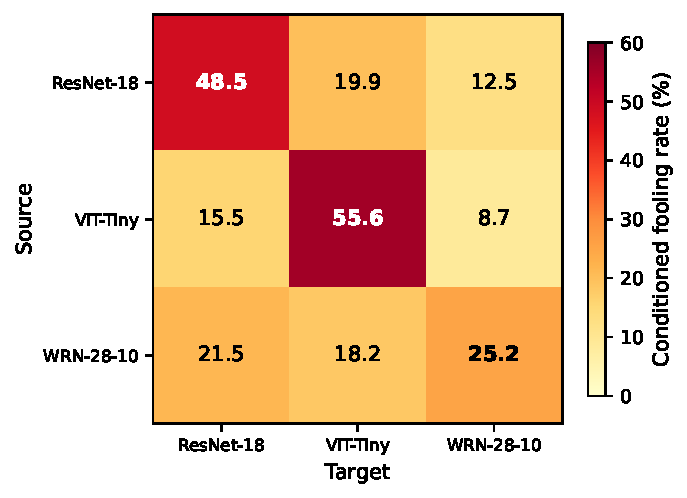
\includegraphics[width=\columnwidth]{../figures/final/fig3_transfer_heatmap.pdf}
\caption{Transfer attack success rate heatmap. CNN-generated adversarial examples transfer to ViT at 41.2\%, while ViT-generated examples transfer to CNN at 36.1\%, revealing a moderate but consistent asymmetry.}
\label{fig:transfer_heatmap}
\end{figure}

Figure~\ref{fig:transfer_heatmap} visualizes this transfer asymmetry.

% ----------------------------------------------------------------------------
% 4.3 Gradient Analysis
% ----------------------------------------------------------------------------
\subsection{Gradient Characteristics}
\label{subsec:gradient}

To explain the transfer asymmetry, we analyze the gradient properties of both architectures. Table~\ref{tab:gradient} summarizes the key gradient statistics.

\begin{table}[!t]
\centering
\caption{Gradient Characteristics Comparison}
\label{tab:gradient}
\begin{tabular}{lcc}
\toprule
\textbf{Metric} & \textbf{ResNet-18 AT} & \textbf{ViT-Tiny AT} \\
\midrule
$L_2$ Norm (mean) & 0.0189 & 0.0211 \\
$L_\infty$ Norm (mean) & 0.00275 & 0.00418 \\
Sparsity & \textbf{7.24\%} & 4.15\% \\
Gradient Alignment & 0.053 & \textbf{0.055} \\
\bottomrule
\end{tabular}
\end{table}

The gradient analysis reveals architectural differences that partially explain the observed transfer asymmetry. CNN gradients exhibit 1.7$\times$ higher sparsity (7.24\% vs 4.15\% near-zero components), indicating more localized sensitivity concentrated around edges and textures. Notably, cross-sample gradient alignment is nearly identical between architectures (0.053 vs 0.055 average pairwise cosine similarity), suggesting that alignment alone does not account for the transfer asymmetry. ViT gradients have 52\% higher $L_\infty$ norm (0.00418 vs 0.00275), indicating larger gradient peaks that attackers can exploit. The sparsity difference, rather than alignment, emerges as the more informative gradient characteristic: sparse CNN gradients concentrate perturbation energy on localized, generic image features---edges, textures, and contours---that both architectures rely on for recognition. ViT gradients, being more uniformly distributed, produce perturbations that spread across the input and are less effective at targeting the localized features that CNN processing depends on.

\begin{figure}[!t]
\centering
\begin{subfigure}[b]{0.48\columnwidth}
    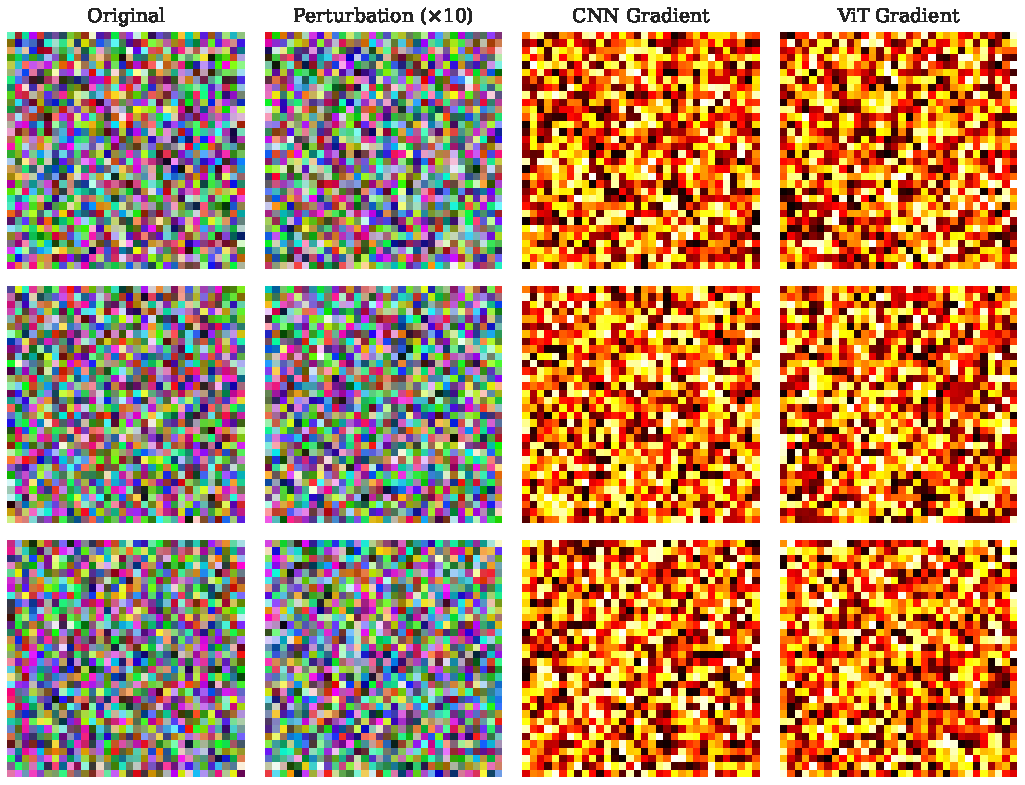
\includegraphics[width=\textwidth]{../figures/final/fig4a_gradient_visualization.pdf}
    \caption{Gradient field visualization}
    \label{fig:gradient_viz}
\end{subfigure}
\hfill
\begin{subfigure}[b]{0.48\columnwidth}
    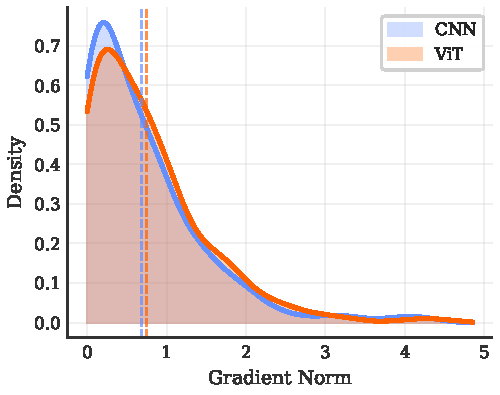
\includegraphics[width=\textwidth]{../figures/final/fig4b_gradient_distribution.pdf}
    \caption{Gradient magnitude distribution}
    \label{fig:gradient_dist}
\end{subfigure}
\caption{Gradient characteristics comparison. (a) CNN gradients exhibit sparse, localized patterns. (b) The gradient magnitude distribution confirms higher sparsity in CNN.}
\label{fig:gradient_analysis}
\end{figure}

Figure~\ref{fig:gradient_analysis} provides visual evidence for these gradient differences.

\begin{figure}[!t]
\centering
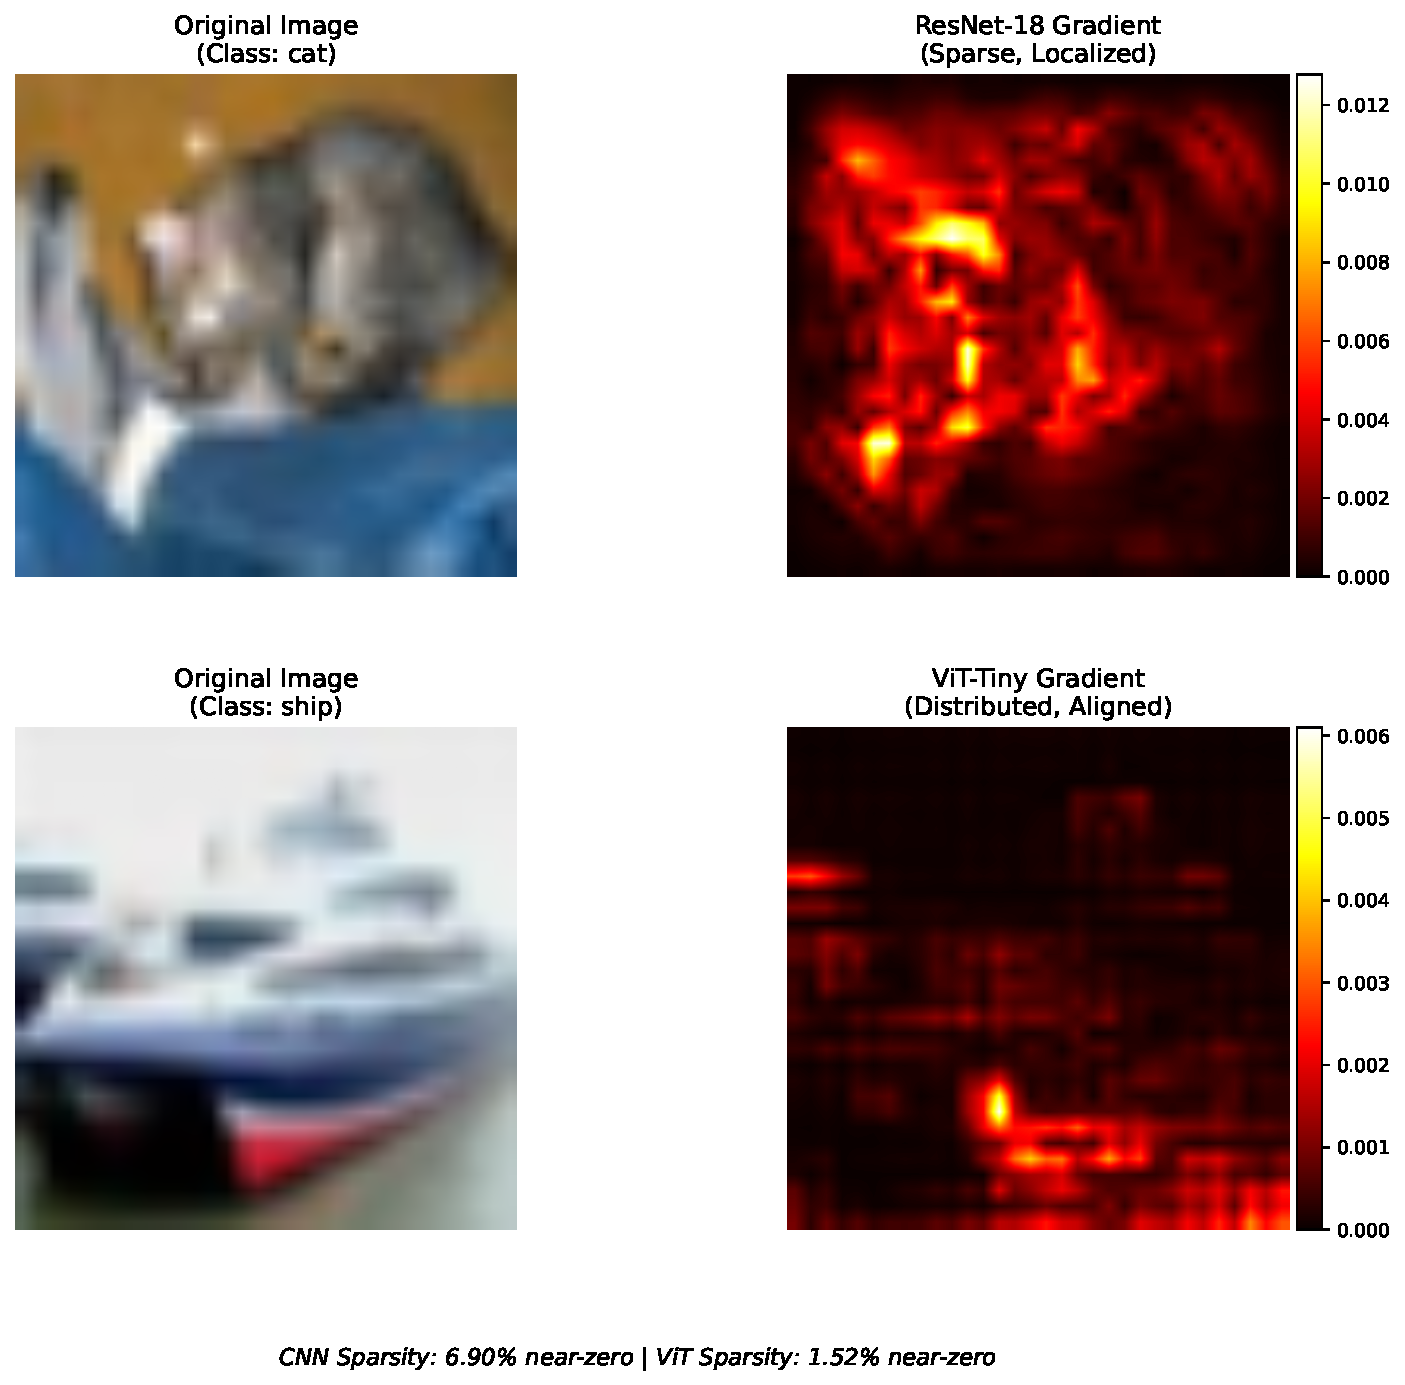
\includegraphics[width=\columnwidth]{../figures/final/fig4_gradient_comparison.pdf}
\caption{Gradient heatmap comparison between CNN and ViT. CNN gradients (top) exhibit sparse, localized patterns concentrated around object edges, while ViT gradients (bottom) are distributed across the entire image with higher alignment across samples.}
\label{fig:gradient_heatmap}
\end{figure}

Figure~\ref{fig:gradient_heatmap} shows a direct comparison of gradient heatmaps, highlighting the structural differences in how each architecture computes input gradients.

% ----------------------------------------------------------------------------
% 4.4 Feature Degradation Analysis
% ----------------------------------------------------------------------------
\subsection{Feature Degradation in Vision Transformers}
\label{subsec:attention}

We analyze how adversarial perturbations affect ViT feature representations across layers. Table~\ref{tab:feature_degradation} shows the layer-wise analysis.

\begin{table}[!t]
\centering
\caption{ViT-Tiny Feature Degradation Under PGD-10 Attack}
\label{tab:feature_degradation}
\begin{tabular}{lccc}
\toprule
\textbf{Layer} & \textbf{$L_2$ Distance} & \textbf{Cosine Sim.} & \textbf{Norm Change} \\
\midrule
\multicolumn{4}{l}{\textit{Early Layers}} \\
Block 0 & 2.57 & 0.995 & $-$0.12\% \\
Block 1 & 1.73 & 0.994 & $-$0.16\% \\
Block 2 & 1.68 & 0.981 & $-$1.18\% \\
\midrule
\multicolumn{4}{l}{\textit{Late Layers}} \\
Block 9 & 1.95 & 0.963 & $-$0.57\% \\
Block 10 & 1.95 & \textbf{0.958} & $-$0.86\% \\
Block 11 & 2.21 & 0.964 & $\mathbf{-1.18\%}$ \\
\bottomrule
\end{tabular}
\end{table}

The layer-wise analysis reveals a progressive feature degradation pattern in ViT layers. Cosine similarity between clean and adversarial features decreases from 0.995 in early layers to 0.958 at Block~10, indicating that adversarial perturbations cause increasing semantic deviation as they propagate through the network. Feature norm changes remain modest throughout, with the largest reduction of $-$1.43\% occurring at Block~5 and $-$1.18\% at Block~11. The degradation is subtler than might be expected given the attack's effectiveness, suggesting that even small directional shifts accumulate into meaningful semantic corruption across twelve transformer blocks. Cosine similarity partially recovers in the final block (Block~11: 0.964), which may reflect the classifier head's regularizing effect on the last transformer block's representations. The early and late layers exhibit qualitatively different behaviors: early layers show high $L_2$ distance but preserved semantic direction (cosine similarity above 0.99), while late layers show smaller absolute changes that nonetheless cause larger directional deviation. This pattern indicates that adversarial perturbations produce a progressive ``semantic drift'' through the ViT feature hierarchy, where small per-layer directional changes compound into sufficient deviation to cause misclassification. A limitation of this analysis is the absence of a comparable layer-wise study for CNN, which would help establish whether this degradation pattern is ViT-specific or a general property of deep networks under adversarial attack.

\begin{figure}[!t]
\centering
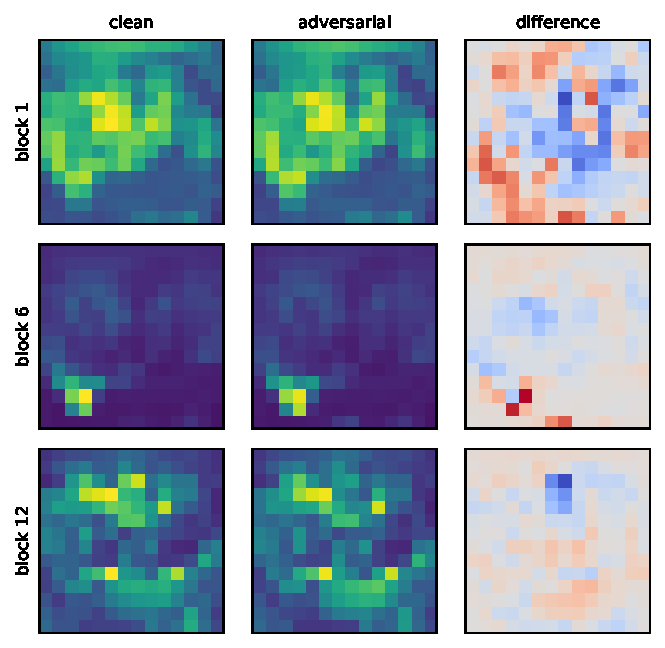
\includegraphics[width=\columnwidth]{../figures/final/fig5_attention_comparison.pdf}
\caption{Attention map comparison across ViT layers under adversarial attack. Each row shows a different layer (1, 6, 12). Columns show clean attention, adversarial attention, and their difference. Early layers maintain similar attention patterns, while late layers show significant attention degradation.}
\label{fig:attention_layers}
\end{figure}

\begin{figure}[!t]
\centering
\begin{subfigure}[b]{0.48\columnwidth}
    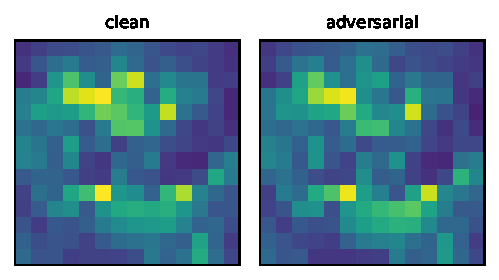
\includegraphics[width=\textwidth]{../figures/final/fig5a_attention_comparison.pdf}
    \caption{Feature degradation heatmap}
    \label{fig:attention_comparison}
\end{subfigure}
\hfill
\begin{subfigure}[b]{0.48\columnwidth}
    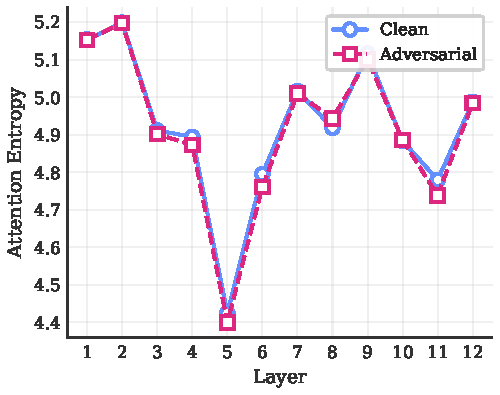
\includegraphics[width=\textwidth]{../figures/final/fig5b_attention_entropy.pdf}
    \caption{Layer-wise metrics}
    \label{fig:attention_entropy}
\end{subfigure}
\caption{ViT feature degradation analysis showing the semantic drift phenomenon.}
\label{fig:feature_degradation}
\end{figure}

Figure~\ref{fig:feature_degradation} visualizes this progressive degradation pattern.

\begin{figure}[!t]
\centering
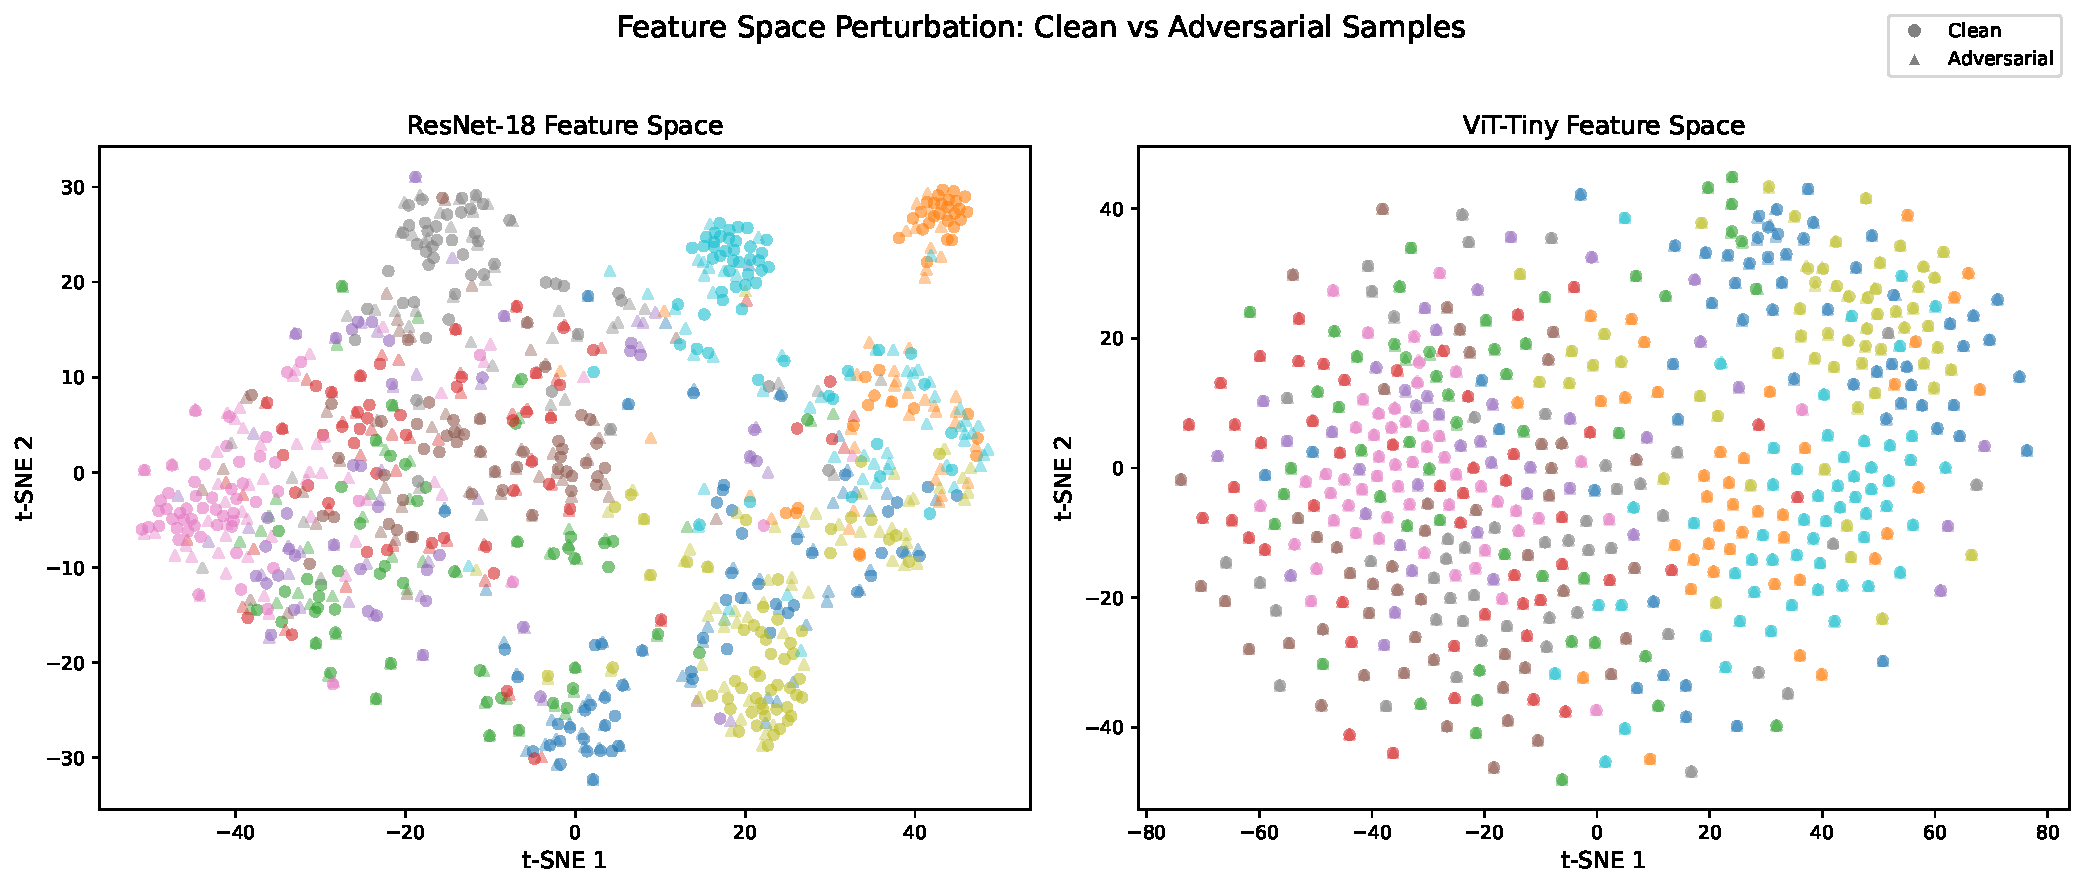
\includegraphics[width=\columnwidth]{../figures/final/fig_tsne_features.pdf}
\caption{t-SNE visualization of feature space perturbation. Clean samples (circles) vs adversarial samples (triangles) for ResNet-18 (left) and ViT-Tiny (right). Adversarial perturbations cause feature displacement that differs between architectures: CNN features show more class-coherent displacement, while ViT features exhibit greater inter-class confusion.}
\label{fig:tsne_features}
\end{figure}

Figure~\ref{fig:tsne_features} provides a t-SNE visualization of how adversarial perturbations affect the learned feature space. The visualization reveals that adversarial examples shift features away from their original class clusters, with different displacement patterns for each architecture.

% ----------------------------------------------------------------------------
% 4.5 Statistical Validation
% ----------------------------------------------------------------------------
\subsection{Statistical Validation}
\label{subsec:statistics_results}

To quantify evaluation stochasticity, we evaluate each trained model across 3 different random seeds (42, 123, 456) for attack initialization on 1,000 test samples. Table~\ref{tab:statistical} shows the results.

\begin{table}[!t]
\centering
\caption{Statistical Validation (Mean $\pm$ Std over 3 evaluation seeds)}
\label{tab:statistical}
\begin{tabular}{lcc}
\toprule
\textbf{Model} & \textbf{Clean Acc (\%)} & \textbf{PGD-10 Acc (\%)} \\
\midrule
ResNet-18 AT & 80.10 $\pm$ 0.00 & 40.03 $\pm$ 0.12 \\
ViT-Tiny AT & 74.00 $\pm$ 0.00 & 37.43 $\pm$ 0.21 \\
\bottomrule
\end{tabular}
\end{table}

The low variance confirms that evaluation stochasticity is negligible. Clean accuracy shows zero variance because the same trained model is evaluated deterministically; variance arises only from random elements in attack initialization and data ordering. Robust accuracy shows minimal variance ($\pm$0.12\% for CNN, $\pm$0.21\% for ViT), indicating stable attack behavior across random seeds.

Beyond evaluation seeds, we additionally conducted two independent training runs (run1 and run2) for each architecture. ResNet-18 AT achieved 40.25\% and 40.97\% PGD-10 accuracy across runs, while ViT-Tiny AT achieved 32.77\% and 36.87\%, respectively. The consistent ranking and comparable magnitudes across runs support the reliability of the observed robustness patterns, though we acknowledge that the training-level variance---particularly for ViT---is larger than the evaluation-level variance reported above.

\textbf{Computational Details:} All experiments were conducted on an NVIDIA RTX 5060 Ti (16GB VRAM) using PyTorch 2.6.0 with CUDA 12.8. AutoAttack evaluation used the standard configuration (APGD-CE, APGD-T, FAB-T, Square) on 500 samples, requiring approximately 13 minutes for ResNet-18 and 22 minutes for ViT-Tiny.
